\begin{center}
    \textbf{ВВЕДЕНИЕ}
\end{center}
\addcontentsline{toc}{chapter}{ВВЕДЕНИЕ}
В современном мире информационные технологии развиваются ежегодно, и для обработки данных требуется больше эффективных методов. Одним из таких методов является параллельная обработка данных с использованием конвейерного подхода~\cite{tanvar_parallel_programming}. Это означает, что весь процесс обработки состоит из нескольких этапов, которые выполняются одновременно, благодаря этому выполнение программы происходит быстрее и ресурсы компьютера используются эффективнее.

Конвейерный подход находит применение в задачах, где необходимо обработать большие объёмы данных, например, при анализе информации, потоковой обработке видео или автоматической обработке данных из различных источников. Данный метод помогает значительно ускорить вычисления.

Целью данной лабораторной работы являются освоение принципов параллельных вычислений на основе конвейерного подхода и разработка программного обеспечения для многократной обработки данных на нескольких этапах.
Для достижения поставленной цели необходимо выполнить следующие задачи:
\begin{itemize}
    \item определить входные и выходные данные;
    \item исследовать особенности параллельной обработки задач;
    \item разработать алгоритмы для обработки данных в конвейерном режиме (чтение данных, их обработка и запись результатов);
    \item реализовать программу с использованием потоков для каждой стадии обработки, включая потоки--генераторы задач и потоки--накопители задач;
    \item провести тестирование разработанных алгоритмов;
    \item сравнить скорость работы программы при различном количестве потоков.
\end{itemize}

\newpage
\aasection{Входные и выходные данные}{sec:input-output}

Программа принимает на вход URL кулинарного веб--сайта и количество страниц для загрузки~\cite{eda_menu}. Входные данные представляют собой HTML файлы с вёрсткой страниц рецептов. Результатом работы программы являются HTML файлы с исходной структурой страниц, а также данные о времени выполнения обработки каждого этапа.


\aasection{Преобразование входных данных в выходные}{sec:algorithm}

Программа получает URL веб--ресурса и извлекает HTML контент с первой страницы. Загруженный код сохраняется в строковой переменной. После этого выполняется анализ содержимого на наличие ссылок на другие страницы рецептов. При нахождении таких ссылок программа осуществляет повторные запросы, извлекая HTML страницы для дальнейшей обработки. Для обработки данных используются параллельные потоки:
\begin{itemize}
    \item Поток для чтения данных из файлов, создаёт задачи на чтение и помещает их в очередь;
    \item Поток для извлечения необходимого подмножества данных (рецептов);
    \item Поток для сохранения извлечённых данных в базу данных.
\end{itemize}
Каждый поток использует очередь для получения задач с входных данных и перемещает результаты в выходную очередь по завершении обработки.

\section{Структура задачи}

Для каждого рецепта сохраняются следующие данные:
\begin{itemize}
    \item \texttt{id} -- уникальный идентификатор задачи на обработку рецепта.
    \item \texttt{issue\_id} -- номер задачи из системы управления проектами.
    \item \texttt{url} -- URL страницы рецепта.
    \item \texttt{title} -- название рецепта.
    \item \texttt{ingredients} -- массив ингредиентов, каждый элемент которого представлен в виде словаря.
    \item \texttt{steps} -- массив шагов приготовления рецепта.
    \item \texttt{image\_url} -- URL изображения рецепта (если имеется).
\end{itemize}


\section{База данных}

Информация о рецептах сохраняется в базе данных, которая поддерживает выполнение SQL запросов и экспорт данных в JSON. Для работы с базой данных использована технология PostgreSQL.


\aasection{Пример работы программы}{sec:demo}

На рисунке~\ref{img:menu} представлен пример работы программы.

\FloatBarrier
\includeimage
{menu} 
{f} % Обтекание (без обтекания)
{h} % Положение рисунка (см. figure из пакета float)
{\textwidth} % Ширина рисунка
{Пример работы программы} % Подпись рисунка
\FloatBarrier
\newpage
На рисунке~\ref{img:bd} представлен пример базы данных \texttt{recipes}, сохранённой в файле \texttt{recipes.db}.
\FloatBarrier
\includeimage
{bd} 
{f} % Обтекание (без обтекания)
{h} % Положение рисунка (см. figure из пакета float)
{\textwidth} % Ширина рисунка
{База данных \texttt{recipes}}
\FloatBarrier

На рисунке~\ref{img:db} представлено продолжение примера базы данных \texttt{recipes}, сохранённой в файле \texttt{recipes.db}.
\FloatBarrier
\includeimage
{db} 
{f} % Обтекание (без обтекания)
{h} % Положение рисунка (см. figure из пакета float)
{\textwidth} % Ширина рисунка
{База данных \texttt{recipes} продолжение}
\FloatBarrier


\aasection{Тестирование}{sec:tests}
В таблице~\ref{tbl:tests} представлены тестовые случаи для системы, которая осуществляет загрузку веб--страниц с указанных URL адресов, обрабатывая их как поочерёдно, так и параллельно, с дальнейшим извлечением данных.

\begin{longtable}{|p{.05\textwidth - 2\tabcolsep}|p{.33\textwidth - 2\tabcolsep}|p{.33\textwidth - 2\tabcolsep}|p{.19\textwidth - 2\tabcolsep}|}
    \caption{Функциональные тесты}\label{tbl:tests} \\\hline
    № теста & Входные данные & Ожидаемый результат & Результат теста \\\hline
    \endfirsthead
    \caption{Функциональные тесты (продолжение)} \\\hline
    № теста & Входные данные & Ожидаемый результат & Результат теста \\\hline
    \endhead
    \endfoot
    1 & Нажатие клавиши \texttt{Enter} &
    Страницы загружаются, данные сохраняются в \texttt{recipes.db} &
    Пройден \\\hline
    2 & Потеря интернет соединения &
    Появляется ошибка при попытке загрузить страницы &
    Пройден \\\hline
    3 & Отключение интернета во время работы программы &
    Ошибка при попытке загрузить страницы &
    Пройден \\\hline
    4 & Загрузка правильного HTML файла &
    Файл загружается и начинается извлечение данных &
    Пройден \\\hline
    5 & Подача пустого HTML файла &
    Появляется ошибка, обработка файла не продолжается &
    Пройден \\\hline
    6 & Подача HTML файла с ошибками в данных &
    Появляется ошибка, данные не извлекаются &
    Пройден \\\hline
    7 & Обработка 10 HTML файлов одновременно &
    Данные извлекаются и сохраняются в базу данных успешно &
    Пройден \\\hline
    8 & Прерывание соединения с базой данных перед сохранением данных &
    Появляется ошибка, данные не сохраняются в базе &
    Пройден \\\hline
\end{longtable}

\aasection{Описание исследования}{sec:study}

В ходе исследования программы для обработки данных веб--страниц с использованием многозадачности фиксируются моменты времени начала и конца обработки задачи на каждом этапе конвейера. Программа разделяет процесс на несколько этапов: чтение данных, извлечение данных и запись данных. Для каждой стадии создаётся отдельный поток, который выполняет свою задачу. Данные передаются между стадиями через очереди.

Для получения следующих характеристик необходимо выполнить следующие измерения:
\begin{itemize}
    \item Среднее время существования задачи;
    \item Среднее время ожидания задачи в каждой из очередей;
    \item Среднее время обработки задачи на каждой из стадий.
\end{itemize}


\section{Технические характеристики}
Технические характеристики используемого устройства:
\begin{itemize} 
    \item операционная система: macOS Monterey;
    \item оперативная память: 8 ГБ;
    \item процессор: Quad-Core Intel Core i5.
\end{itemize}

\section{Результаты исследования}
В результате исследования получены следующие данные:
\begin{itemize}
    \item 4150 миллисекунд — среднее время существования задачи;
    \item 1200 миллисекунд — среднее время в очереди на чтение данных;
    \item 1700 миллисекунд — среднее время в очереди на извлечение данных;
    \item 1400 миллисекунд — среднее время в очереди на запись данных;
    \item 7 миллисекунд — среднее время чтения данных;
    \item 5 миллисекунд — среднее время извлечения данных;
    \item 4 миллисекунды — среднее время записи данных.
\end{itemize}

В таблице~\ref{tbl:time_measurements2} представлены среднее время работы и среднее время простоя для каждого этапа обработки данных, измеренные в секундах.
\begin{table}[h]
    \begin{center}
        \begin{threeparttable}
        \captionsetup{justification=raggedright,singlelinecheck=off}
            \caption{Среднее время работы и простоя на каждом этапе обработки данных (в секундах)}
            \label{tbl:time_measurements2}
            \resizebox{\textwidth}{!}{
                \begin{tabular}{|r|r|r|}
                    \hline
                    Название этапа & Среднее время работы (с) & Среднее время простоя (с) \\
                    \hline
                    \texttt{read\_stage} (чтение данных) & 1.7500 & 0.0000 \\
                    \texttt{extract\_stage} (извлечение данных) & 0.0930 & 1.7000 \\
                    \texttt{store\_stage} (запись данных) & 0.0140 & 1.7500 \\
                    \hline
                \end{tabular}
            }
        \end{threeparttable}
    \end{center}
\end{table}

\section*{Вывод}  
В процессе параллельной обработки данных часть времени уходит на простои, а не на выполнение операций.  

Этап чтения данных (\texttt{read\_stage}) выполняется за 1.7500 секунд и не имеет времени простоя, так как выполняется непрерывно. Этап извлечения данных (\texttt{extract\_stage}) демонстрирует минимальное время выполнения (0.0930 секунды), но обладает длительным временем простоя (1.7000 секунды) из-за ожидания данных. Этап записи данных (\texttt{store\_stage}) выполняется быстрее всего (0.0140 секунды), но время его простоя достигает 1.7500 секунды, что связано с задержками на предыдущих этапах.  

Таким образом, основная проблема заключается в больших простоях на разных этапах обработки, что снижает общую производительность.  Чтение и обработка HTML данных является сложным процессом, где длительное время тратится на ожидание. Для повышения эффективности лучше использовать заранее подготовленные данные.

% На рисунке~\ref{fig:graph1} показано, как изменяется время выполнения при увеличении числа потоков, при постоянном количестве обрабатываемых страниц.

% \begin{figure}[h!]
%     \centering
%     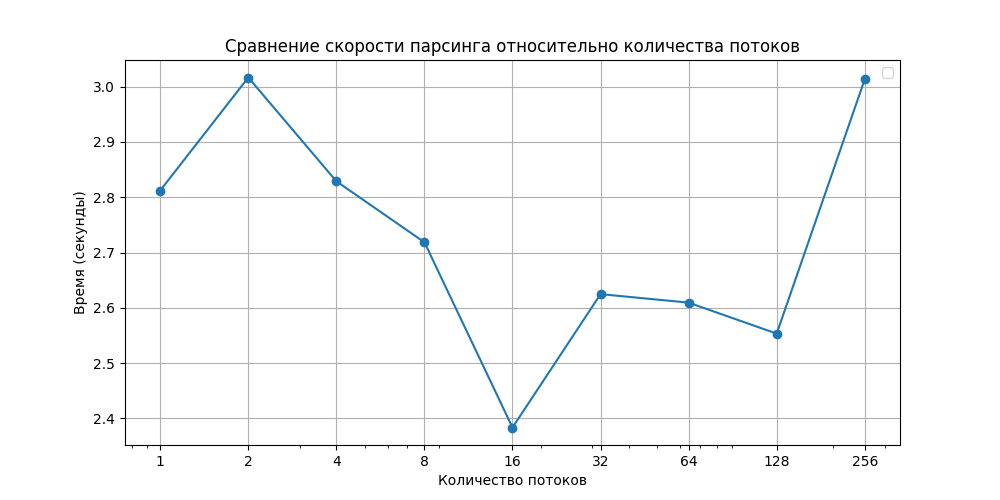
\includegraphics[scale=0.6]{inc/img/graph1.png}
%     \caption{Зависимость времени выполнения программы от количества потоков}
%     \label{fig:graph1}
% \end{figure}
% \clearpage

\clearpage
\aaunnumberedsection{ЗАКЛЮЧЕНИЕ}{sec:outro}

Цель лабораторной работы была достигнута. В ходе выполнения работы решены следующие задачи:

\begin{itemize}
    \item определены входные и выходные данные для обработки в рамках конвейерного подхода;
    \item исследованы особенности параллельной обработки задач, включая влияние числа потоков на производительность;
    \item разработаны алгоритмы для обработки данных в конвейерном режиме, включающие этапы чтения, обработки и записи данных;
    \item реализована программа с использованием потоков для каждой стадии обработки данных, включая потоки-генераторы задач и потоки-накопители задач;
    \item проведено тестирование разработанных алгоритмов с оценкой их эффективности по времени и памяти;
    \item проведено сравнение скорости работы программы при различном количестве потоков.
\end{itemize}

Исследования показали, что параллельные вычисления значительно ускоряют выполнение задач, особенно на этапах, требующих больших вычислительных ресурсов. При увеличении числа потоков производительность растёт до определённого предела, после чего прирост становится менее заметным. Это связано с ограничениями оборудования и дополнительными затратами на управление потоками.

Анализ временных показателей показал, что значительная часть времени уходит на ожидание данных между этапами обработки. Снижение этих задержек может повысить эффективность работы программы. Таким образом, использование конвейерного подхода подтверждает эффективность для задач, требующих многозадачной обработки.

